\cleardoublepage
\chapter{GLSL}
\label{ch:12}
 
%------------------------------------------------

\section{Introduction}

\begin{fullwidth}
GLSL, or OpenGL Shading Language, is an incredible tool to have in one's back pocket. With a little bit of code, one can program directly on the GPU. 

Many avoid learning GLSL because they believe that it is only useful for working with large textures (4K and beyond), complex 2D generative visual scenes, or creating and manipulating 3D geometry, but it can be used in so many facets of day to day programming. Whether that be optimizing and creating incredibly effecient compositing workflows for standard HD content, or creating simple generative backgrounds for interactive experiences. 

The goal of this chapter is to introduce the reader to some basic GLSL workflows and techniques, with the assumption that the reader has no previous GLSL experience. 

\end{fullwidth}

%------------------------------------------------

\section{Types of Shaders and Rendering Pipeline}

\begin{fullwidth}
The two main types of shaders that can be programmed in TouchDesigner are the Vertex shader and the Pixel (or Fragment) shader. In a standard rendering pipeline, they are processed in that order, as can be seen in the diagram below:

\begin{center} 
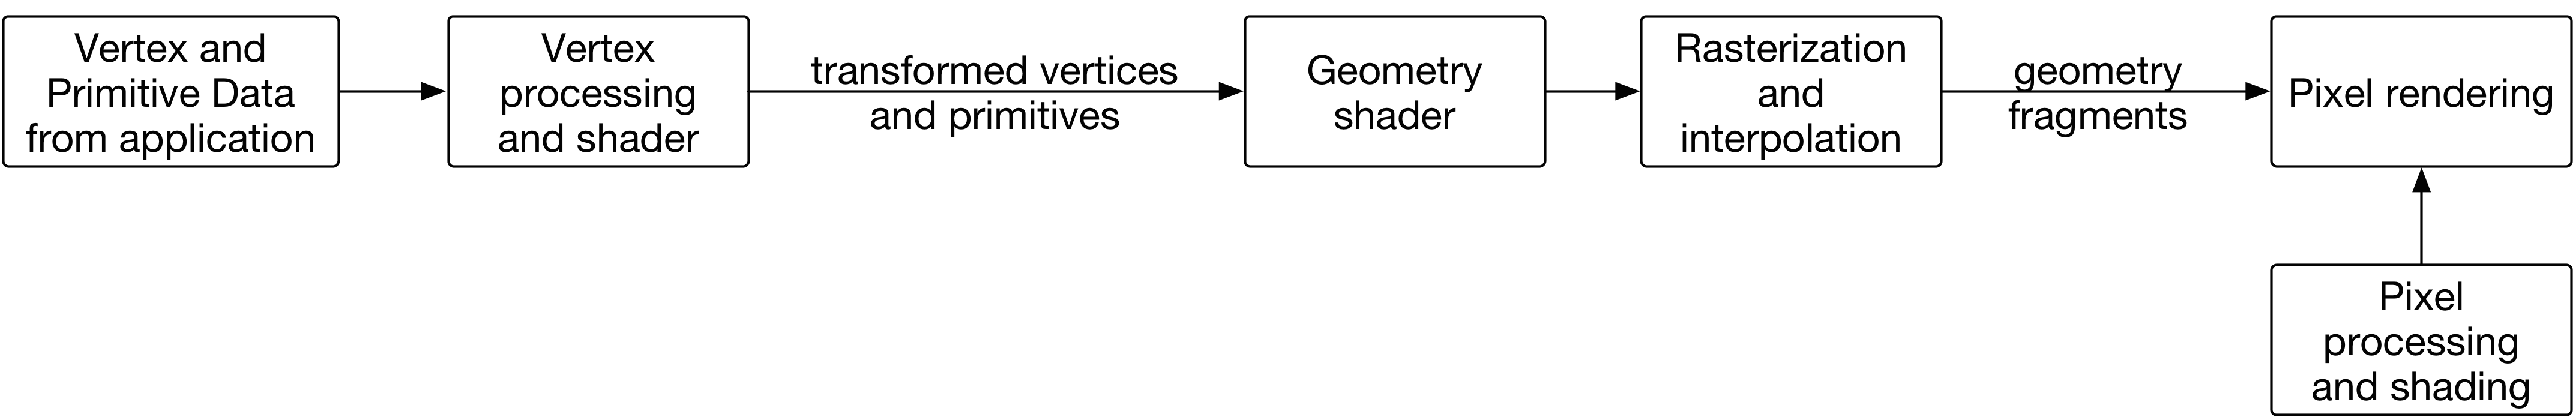
\includegraphics{./img/12.2/pipeline.png}
\end{center}

There is also a geometry shader that can be applied between the Vertex and Pixel shaders for layered rendering and transform feedbacks, but it is not used commonly.

In the above pipeline, the application passes the vertex and primitive data to the GPU. This includes information such as vertex position, texture coordinate, color, normal, etc. This information can be programatically processed and worked with by using a Vertex shader.

When the Vertex shader has finished processing the vertex and primitive data, the geometry is rasterized. During this process, the geometry goes through various stages such as clipping, culling, transformations to window space, etc. These stages prepare fragments that will be processed by the Pixel shader. 

The Pixel shader takes these fragments, processes them, and outputs the color and depth data for each pixel.

For a more in-depth look at the render pipeline, there is a more thorough explanation on the OpenGL website:

\url{http://www.opengl.org/wiki/Rendering_Pipeline_Overview}
 
\end{fullwidth}

%------------------------------------------------

\section{Debugging}

\begin{fullwidth}
Before getting too deep into the world of GLSL, it is important to know how to debug compiling issues. There are two signs that denote a compiling error. 

The first is a blue and red checker pattern. When working with the GLSL MAT, this check pattern will be on the geometry itself. When using GLSL with TOPs, this checker pattern will fill up the Operator's viewer and be output from the TOP.

The second sign of a compile error is a yellow triangle warning flag on the Operator. Upon clicking and holding the left mouse button on the flag, the error will read: 

\begin{lstlisting}
Warning: The GLSL Shader has compile error
\end{lstlisting}

To diagnose these issues, an Info DAT is required. Create an Info DAT, and set the 'Operator' Parameter to reference the GLSL operator with the error. In the Info DAT, if there are no errors, there will be only a few lines and of them will read 'Compiled Successfully' or 'Linked Successfully'. If there are errors however, they will read more like:

\begin{lstlisting}
Pixel Shader Compile Results:
0(3) : error C0000: syntax error, unexpected '=', expecting '::' at token '='
\end{lstlisting}

To quickly break this down, the first thing is the line number. In this case, '0(3)' means the compiler is encountering errors at line 3. In many situations, this may mean that the actual mistake happens a line or two earlier, but the compiler doesn't halt until the next line when things stop making sense for it. 

The next section highlights that this is a syntax error, and then there is more information about the error. 

For beginners, the majority of these errors will be because of forgotten semi-colons at the end of lines, or errors trying to cast one data type into another incompatible data type.


\end{fullwidth}

%------------------------------------------------

\section{Shaders in 3D}

\begin{fullwidth}
Let's start by looking at a few very simple 3D scenes that utilize Vertex and Pixel shaders. 

Open example 'Basic\_3D.toe'. 

This is a simple render setup where the vertex shader does nothing but pass the vertices to the pixel shader, which then colors everything white. Let's take a more in-depth at each shader, starting with the Vertex shader:

\begin{lstlisting}
void main(){
	gl_Position = TDWorldToProj(TDDeform(P));
}
\end{lstlisting}

Since this is written for someone with no GLSL experience, a few notes about basic C syntax and rules that need to be followed, since GLSL is very similar to C.

The first thing is that semi-colons need to be added at the end of working lines of code. 

The second thing is that most of the working code will be inside of the main() loop. For beginners, the only things outside of the main loops will be the delcaring of variables such as input and output streams and attributes. 

When starting an empty shader, it's good practice to start by entering the main() loop as follows:

\begin{lstlisting}
void main(){
	
}
\end{lstlisting}

In this vertex shader, there is only have one line of code:

\begin{lstlisting}
gl_Position = TDWorldToProj(TDDeform(P));
\end{lstlisting}

Let's break this down from right to left, as there is a lot going on here. 

'P' in this instance is the vertex position. In TouchDesigner, there are a few attributes that are declared by default. For instance, 'P' is the vertex position, 'N' is the normal, 'Cd' is the color, and 'uv' is the texture coordinate layers (it is an array that is accessed by index, i.e. uv[0], uv[1], etc). These values can be accessed as easily as we've accesed 'P'.

In the line of code, 'P' is input into a function named 'TDDeform()'. This function takes the vertex position from object space and returns the position in world space. 

Think of object space as if each object in the 3D world had it's own co-ordinate system and 0,0,0 point. After processing these vertices, they have to be transformed and integrated into world space. World space is, as the name implies, the full world. The world, in this case, is the common coordinate system, with one 0,0,0 point, where all objects will exist together.

Once the vertex positions are returned in world space, they are passed to the function 'TDWorldToProj()'. This function takes the world space co-ordinates and returns them in projection space. The projection space takes all the co-ordinates from the world space, and returns them from a camera's point of view.

These values are then assigned to the variable 'gl\_Position', which is a built-in output for the transformed vertices.

As shown in the rendering pipeline diagram, these transformed vertices are processed and passed to the Pixel shader, where they will be assigned color values.

In this example, the Pixel shader sets the color output of all the fragments to white. The code is below: 

\begin{lstlisting}
out vec4 fragColor;
void main(){
	fragColor = vec4(1,1,1,1);
}
\end{lstlisting}

Similar to the Vertex shader, all of the code except for the output declaration are inside of the main() loop, and there are semi-colons at the end of lines of code. 

Starting from the top, there is this line of code:

\begin{lstlisting}
out vec4 fragColor;
\end{lstlisting}

This line sets the output as a variable called 'fragColor'. A 'vec4' is a vector with 4 components, and in this scenario, they correspond to the output red, green, blue, and alpha channels. In GLSL, whenever declaring an input or output, the type must be declared as well, thus the specification that it will be a 'vec4'. Similarly, inputs will be prefaced by 'in' and outputs will be prefaced by 'out'.

The line of code inside of the main() loop is as follows:

\begin{lstlisting}
fragColor = vec4(1,1,1,1);
\end{lstlisting}

As 'fragColor' has already been declared as the output, this line writes the pixel values directly to the output. The section 'vec4(1,1,1,1)' creates a 4-component vector with the values 1,1,1,1, and then assigns it to 'fragColor'. 'vec4' has to precede the list of values because 'fragColor' has already been declared as a vec4, so to assign a value to it, that value needs to be a 'vec4'. 

Because the 4 components of the output correspond to RGBA channels, (1,1,1,1) would set all of the channels to 1, effectively setting the output to white for every pixel. 

Now with a basic understand of working with shaders in a 3D scene, let's add a few levels of complexity. For starters, let's resize the box. This is as simple as multiplying each of the vertex positions, or 'P', by a value.

Open example 'Basic\_3D\_scaled.toe'. 

Only a few lines of the vertex shader are changed:

\begin{lstlisting}
vec3 scaledP;

void main(){
	scaledP = P * 0.5;
	gl_Position = TDWorldToProj(TDDeform(scaledP));
}
\end{lstlisting}

The first this that is added is a declaration for a variable that is going to be used, named 'scaledP'. This is going to be a 3-component vector because we'll be working with the vertex position, 'P', which is also a 3-component vector. 

Once the variable is defined, it can be used throughout the code. The next line that is added is:

\begin{lstlisting}
scaledP = P * 0.5;
\end{lstlisting}

This line takes the vertex position, multiplies all the values by 0.5, effectively making the box half the size. Similarly, a value of 2 would make the box be double it's original size. 

This new value, 'scaledP', then replaces 'P' below:

\begin{lstlisting}
gl_Position = TDWorldToProj(TDDeform(scaledP));
\end{lstlisting}

Similarly, to transform the box instead of scaling it, values need to be added or subtracted to the various axis. 

Open example 'Basic\_3D\_transform.toe'.

In this example, The code in the vertex shader has been changed as below:

\begin{lstlisting}
vec3 transformedP;

void main(){
	transformedP = P + vec3(1,0,0);
	gl_Position = TDWorldToProj(TDDeform(transformedP));
}
\end{lstlisting}

This is very similar to the above example. It starts off by declaring a 3-component vector named 'transformedP'. In the first line of the main() loop, instead of multiplying the vertex positions by 0.5, the new 3-component vector is being added to them. 

The reason to use a 'vec3' in this example is that if 0.5 was simply added to 'P', it would add 0.5 to the x-axis, 0.5 to the y-axis, and 0.5 to the z-axis. Creating a 'vec3' for these values allows control over each specific axis. In this example, adding 'vec3(1,0,0)' will only add 1 to the x-axis, leaving the y-axis and z-axis untouched. In practice, this moves the box 1 unit to the camera's right.

We could just as easily change from addition to subtraction to move the box in the other direction. 

Now, let's reference an LFO CHOP from the vertex shader to animate the movement.

Open example 'Basic\_3D\_LFO.toe'.

For this to be achieved, an LFO CHOP was created. The value of it's channel was then exported to the GLSL MAT's parameter 'value0x' in the 'Vectors 1' tab of the Parameter window. Then the Uniform was given a name, in this case 'lfoCHOP'. This means the value can now be accesed from within the vertex and pixel shaders. 

The code in the vertex shader has been changed as follows:

\begin{lstlisting}
vec3 transformedP;
uniform float lfoCHOP;

void main(){
	transformedP = P + vec3(lfoCHOP,0,0);
	gl_Position = TDWorldToProj(TDDeform(transformedP));
}
\end{lstlisting}

The first addition is in the second line, where a 'uniform' is declared. A 'uniform' is a global GLSL variable that is mainly used for parameters that a user or program will pass into the shader.

In this example, the LFO CHOP channel is a float value, so then 'float' is added after 'uniform'. The name of the uniform is important, because it must correspond to the name entered in the 'Uniform Name' parameter in the GLSL MAT. In the GLSL MAT, we named the uniform 'lfoCHOP', so to access it, the same name must be used.

The only other change is that where previously 1 was being added to the x-axis of the vertex position, there is now the value of 'lfoCHOP'.

\begin{lstlisting}
transformedP = P + vec3(lfoCHOP,0,0);
\end{lstlisting}

With those small changes, a CHOP is controlling the x-axis position of the shader. Pixel shaders function in much of the same way as Vertex shaders. Let's assign the LFO CHOP in the previous example to control the red channel of the output color. 

Open example 'Basic\_3D\_red.toe'.

In this example, the LFO CHOP is controlling the red channel of the pixel shader in much the same way that the LFO CHOP is controlling the x-axis transform.

The code in the Pixel shader is below:

\begin{lstlisting}
out vec4 fragColor;
uniform float lfoCHOP;

void main(){
	fragColor = vec4(lfoCHOP,0,0,1);
}
\end{lstlisting}

Similarly to the x-axis transform example, the only steps needed were to declare the incoming uniform, and then to assign it to a parameter, in this case the first component of the vector. To take this another step furtuer, let's sample a Ramp TOP as the texture, instead of just outputting a single color. 

Open example 'Basic\_3D\_texture.toe'.

The first thing that was done was create the Ramp TOP and assign it to the GLSL MAT. The TOP needs to be referenced in the 'Samplers 1' tab in the Paramter window. In the same way that the LFO CHOP needed a 'Uniform Name', the Ramp TOP needs a 'Sampler Name', which in this case is 'rampTOP'.

Then a Texture SOP is added after the Box SOP to assign the texture co-ordinates.

In the Vertex shader, a few lines of code are added to assign the texture co-ordinates. These lines are added below:


\begin{lstlisting}
vec3 transformedP;
uniform float lfoCHOP;
out vec2 texCoord0;

void main(){
	transformedP = P + vec3(lfoCHOP,0,0);
	gl_Position = TDWorldToProj(TDDeform(transformedP));

	vec3 texCoord = TDInstanceTexCoord(uv[0]);
	texCoord0.st = texCoord.st;
}
\end{lstlisting}

The first line that is added is:

\begin{lstlisting}
out vec2 texCoord0;
\end{lstlisting}

This line outputs a 2-component vector named 'texCoord0' which can be used in the pixel shader. In this case, they will be the texture UV co-ordinates.

There is one more additional line:

\begin{lstlisting}
texCoord0.st = uv[0].st;
\end{lstlisting}

This line takes 'texCoord0' that was declared earlier, and assigns it the built-in TouchDesigner variable 'uv', which as mentioned earlier is declared by default and contains the UV texture co-ordinates (similar to 'P' for vertex position). 

The '.st' here is assigning the two values contained in the 2-component vector 'uv' to the 2 components of 'texCoord0'. As mentioned earlier, where '.xyzw' are used for vertex positions, '.stpq' are often used for texture co-ordinates. These are mostly just for convention so that the same letters (such as XYZW and RGBA) don't mean multiple different things. You may also see '.uv' used instead of '.st', depending on the software package. 

With these two extra lines of code, the Box SOP is now being textured by the Ramp TOP.

\end{fullwidth}

%------------------------------------------------

\section{Shaders in 2D}

\begin{fullwidth}
Even if one doesn't want to spend a ton of time learning about GLSL for 3D use, the Pixel shader can be extremely useful as a tool for generative visuals and compositing 2D textures. Simple GLSL shaders can be especially useful when compositing textures, as it can save quite a lot of graphics memory when doing repititious work.

Let's take a look at an example of adding two TOPs together, similar to a Add TOP.

Open example 'Basic\_2D\_add.toe'.

Using the GLSL TOP, multiple TOP inputs can be composited, sampled, and effected in a GLSL pixel shader. In this example, a Movie In TOP and a Constant TOP are input into the GLSL TOP. The GLSL code in the pixel shader, adds them together:

\begin{lstlisting}
out vec4 fragColor;

void main(){
	vec4 in1 = texture(sTD2DInputs[0], vUV.st);
	vec4 in2 = texture(sTD2DInputs[1], vUV.st);
	fragColor = in1 + in2;
}
\end{lstlisting}

Working with Pixel shaders in the TOP family is very similar to working with them using a GLSL MAT. There is still a main() loop, the declarations happen first before the main() loop, and there are semi-colons at the end of working lines of code.

The first difference to notice is how inputs are handled. In this example there are two inputs, and there are two lines that deal with those inputs:

\begin{lstlisting}
vec4 in1 = texture(sTD2DInputs[0], vUV.st);
vec4 in2 = texture(sTD2DInputs[1], vUV.st);
\end{lstlisting}

To get access to a TOP input, a 4-component variable must be declared for the RGBA channels. The texture() function is used to sample a texture. It takes two arguments, the first is the texture that it is going to sample, which in these cases are TOP inputs. The second argument is the texture co-ordinate to sample.

In this case, since TOP inputs are being sampled, the built-in sampler array named 'sTD2DInputs' is used. This array is accessed by index. In this case, there are two TOP inputs, so 'sTD2DInputs[0]' is used to access the first input, and 'sTD2DInputs[1]' is used to access the second. 

To access the proper texture co-ordinate, 'vUV.st' is used. 'vUV' is a built-in variable that contains the texture co-ordinates of the pixel. As mentioned, '.st' is used to access the first two components of the vector.

Once the appropriate pixel is addressed from each input, this example procedes to add the pixels together, and output them to 'fragColor', which is the defined output:

\begin{lstlisting}
fragColor = in1 + in2;
\end{lstlisting}

As simple as that, a main functionality of the Add TOP has been replicated. This may seem like a round-about way of adding two textures, but the benefits of something as simple as this begin to become apparent when using more complicated workflows or the GLSL Multi TOP, which is fundamentaly the same as the GLSL TOP, except that it has an infinite number of TOP inputs (limited only by the graphics card).

Open example 'Basic\_2D\_multi.toe'.

This example expands on the previous example by adding together more sources. This is done by connecting all the sources into a GLSL Multi TOP, and then accesing them in the same way that the two inputs were accessed previously.

In the shader of this example, each input takes the next index of 'sTD2DInputs' and assigns it to another 'vec4', after which they are all added together.

Again, this might be useful, but a Composite TOP can add multiple inputs s well, so let's take it one step further. 

Open example 'Basic\_2D\_composite.toe'.

This example takes the previous example a step further. With all the inputs defined, instead of just adding all the inputs together, the GLSL code does a mix of addition, subtraction, and multiplication. Remembering the order of operations when working like this is key! 

This is incredibly useful when working with a large number of textures, even if just 1920x1080, because doing a similar process with TOPs would take multiple Composite TOPs, or a number of Multiply, Add, and Subtract TOPs. Being able to manipulate all these textures, even in such simple methods, all at once can save quite a bit of GPU memory.

Transforming the textures is very similar to transforming vertices in a vertex shader. Let's take a look at an example.

Open example 'Basic\_2D\_transform.toe'.

This example takes the previous example, and offsets a few of the textures. This is done by adding, subtracting, multiplying, and dividing the texture co-ordinate. Let's examine the example code below:

\begin{lstlisting}
out vec4 fragColor;

void main(){
	vec4 in1 = texture(sTD2DInputs[0], vUV.st * 0.5);
	vec4 in2 = texture(sTD2DInputs[1], vUV.st);
	vec4 in3 = texture(sTD2DInputs[2], vUV.st - vec2(0.5,0.25));
	vec4 in4 = texture(sTD2DInputs[3], vUV.st);
	vec4 in5 = texture(sTD2DInputs[4], vUV.st + vec2(0.5,0.));

	fragColor = in1 + in2 * in3 - in4 * in5;
}
\end{lstlisting}

In the above example, three of the textures are being transformed. The first is being scaled up by a factor of two. To do this, 'vUV.st' is multiplied by 0.5. This may seem backwards, but remember that 'vUV' is the texture co-ordinates, so when both x-axis and y-axis co-ordinates are moved to the right, the image moves to the left. Imagine having a finger pointing into the center of a piece of paper. If the finger position is moved to the right, the image will be more to the left of the finger than before. This is an overtly simple example, but should help get the idea across.

The third input, 'in3', has been translated on both x-axis and y-axis by subtracting 0.5 from the x-axis, and 0.25 from the y-axis. 

The final input, 'in5', has been translated on the x-axis by adding 0.5 to the x-axis. 

Both of these two tranformations also follow the same thought process mentioned for the first transformation. For example, when adding 0.5 to the x-axis texture co-ordinates, they are being added to the texture co-ordinates and not the position of the image. Thus when the texture co-ordinates move 0.5 on the x-axis, the image appears to move to the left.

The final example will be to take the previous exampleoutputs each individual layer to a separate color buffer instead of compositing them.

Open example 'Basic\_2D\_buffers.toe'.

The shader is as follows:

\begin{lstlisting}
out vec4 fragColor[5];

void main(){
	vec4 in1 = texture(sTD2DInputs[0], vUV.st * 0.5);
	vec4 in2 = texture(sTD2DInputs[1], vUV.st);
	vec4 in3 = texture(sTD2DInputs[2], vUV.st - vec2(0.5,0.25));
	vec4 in4 = texture(sTD2DInputs[3], vUV.st);
	vec4 in5 = texture(sTD2DInputs[4], vUV.st + vec2(0.5,0.));

	fragColor[0] = in1;
	fragColor[1] = in2;
	fragColor[2] = in3;
	fragColor[3] = in4;
	fragColor[4] = in5;

}
\end{lstlisting}

The first line of the shader has been modified so that the output 'fragColor' is now an array. Each component of the array can be assigned a different texture, as has been done at the end of the shader. At which point, with the '\# of Color Buffers' parameter for the GLSL Multi TOP set to 5, Render Select TOPs can be used to individually select each of the separate color buffers from inside of the GLSL Multi TOP using the. To do this, the 'Render or GLSL TOP' parameter references the GLSL Multi TOP, and the 'Color Buffer Index' parameter is set to the target color buffer.

Assigning textures to the color buffers is similar to assigning textures to a single output, with the addition of the color buffer index:

\begin{lstlisting}
fragColor[0] = in1;
\end{lstlisting}

The number in the square brackets refers to the buffer being written to. In the above example, the first buffer is being written to.

\end{fullwidth}

%------------------------------------------------

\section{What Next?}
\begin{fullwidth}
This chapter should have helped unravel a bit of the introductory mysteries of GLSL without getting unnecessarily technical. 

If you'd like to continue learning GLSL to experiment with more complex 3D scenes and material shaders, or with more complex 2D compositing tools and generative textures, below are some resources:

\begin{enumerate}
\item OpenGL Main reference page: \url{http://www.opengl.org/wiki/Main_Page}
\item OpenGL General information: \url{http://www.opengl.org/wiki/General_OpenGL}
\item Derivative Wiki: \url{http://www.derivative.ca/wiki088/index.php?title=Glsl}
\item Shader Toy: \url{https://www.shadertoy.com/}
\end{enumerate}
\end{fullwidth}